\section{A Stage-Resolved Model of Persistent-State Transport}
\label{sec:mechanism}
Let a task $x$ produce trajectory $\tau$ and let the terminal evaluator emit $r\in\{0,1\}$. A reward-conditioned memory writer constructs
\begin{equation}
M_r = G(\tau,r).
\end{equation}
In the released ReasoningBank implementation, $r=1$ selects a success-reflection objective and $r=0$ selects a failure-reflection objective. Our paired intervention holds $\tau$ fixed and changes only the selected writer branch. The first estimand is therefore a persistent-state contrast,
\begin{equation}
D_M(\tau)=d\!\left(M_1,M_0\right),
\end{equation}
where $d$ is a prespecified memory-distance statistic. This quantity answers whether the update surface changes. It does \emph{not} answer whether the changed state is later exposed to the policy or behaviorally consequential.

We therefore decompose downstream transport into three additional stages. For a held-out future state $x'$, let $E_r(x')\in\{0,1\}$ indicate whether branch-specific memory from $M_r$ is retrieved into the future context. Let $A_r(x')$ denote the first structured policy action under that context, and let $Y_r(x')$ denote the terminal task outcome. The stage-specific objects are
\begin{align}
T_E &= \Pr(E_r=1),\\
T_A &= d_A\!\left(P(A\mid M_1,x'),P(A\mid M_0,x')\right),\\
T_Y &= \left|\mathbb{E}[Y\mid M_1,x']-\mathbb{E}[Y\mid M_0,x']\right|.
\end{align}
A large $D_M$ can coexist with a small $T_A$ or $T_Y$ if branch-specific content is rarely retrieved, ignored after retrieval, dominated by the current observation, or behaviorally redundant. This is the core identification point of the paper.

\begin{figure}[t]
\centering
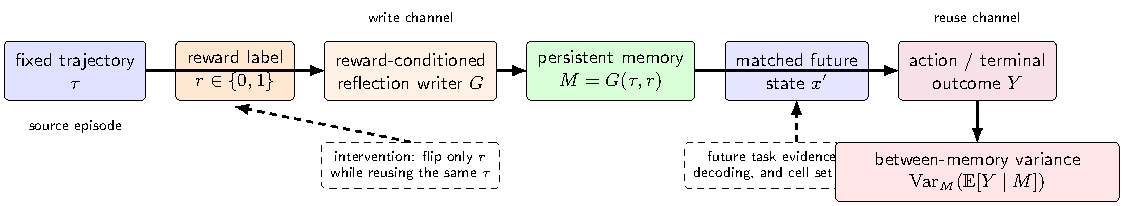
\includegraphics[width=\linewidth]{figures/fig1_reward_write_channel.pdf}
\caption{The stage-resolved reward-to-memory transport chain. The source trajectory is fixed while the terminal reward label selects the released reflection writer. The resulting state must then survive retrieval exposure and policy uptake before it can affect terminal outcome. A forced-memory packet bypasses the native exposure stage and therefore measures downstream \emph{leverage}, not native end-to-end transport.}
\label{fig:write}
\end{figure}

\subsection{Forced leverage versus native transport}
A direct memory injection and a native memory-bank rollout estimate different quantities. In a forced packet, the experimenter supplies $M_r$ to the policy, so exposure is mechanically set to one. The terminal contrast
\begin{equation}
L_Y(x')=\left|\mathbb{E}[Y\mid do(M=M_1),x']-\mathbb{E}[Y\mid do(M=M_0),x']\right|
\end{equation}
asks whether the paired states are \emph{capable} of changing behavior under matched evidence. In native reuse, retrieval remains part of the system, and the end-to-end contrast combines exposure and uptake. Consequently, $L_Y>0$ does not imply a large native $T_Y$.

This distinction resolves an apparent contradiction in our experiments. Forced injection produces a substantial terminal contrast, while native Shopping and Reddit transport is sparse. Rather than choosing one result as the ``real'' effect, the stage model treats both as measurements of different links in the same causal chain.

\subsection{Attenuation as the mechanism diagnostic}
For descriptive comparison, define a stage attenuation ratio whenever the upstream denominator is nonzero,
\begin{equation}
\alpha_{j\rightarrow k}=\frac{T_k}{T_j}.
\end{equation}
We do not interpret this ratio as a universal causal coefficient because the stage metrics use different scales. Its role is diagnostic: it forces the analysis to ask where a large upstream intervention stops being behaviorally expressed. The scientific claim rests on the separately measured stage endpoints and their qualitative ordering, not on a single composite score.

The resulting evaluation principle is simple: \emph{do not infer behavioral authority from persistent-state divergence alone}. An update should be characterized at the write, exposure, uptake, and outcome stages separately, with forced-injection tests used only to establish latent leverage when native transport is weak.
